%
% fig-gitterapprox.tex -- Beweis des Homologie-Satzes
%
% (c) 2026 Prof Dr Andreas Müller
%
\begin{figure}
\centering
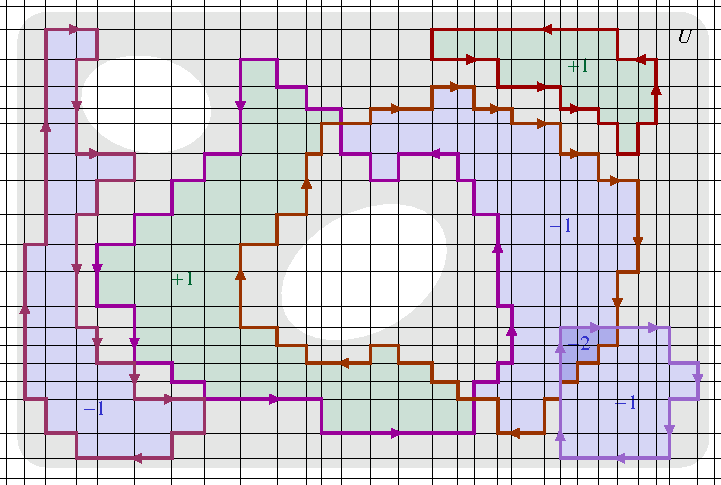
\includegraphics{chapters/030-integration/images/gitterapprox.pdf}
\caption{Eine nullhomologe Kette lässt sich durch eine nullhomologen Kette
$c$ mit achsparallelen Segmenten approximieren, ohne dass sich
Integrale ändern.
Die Segmente definieren eine Unterteilung der Ebene in Rechtecke.
Jedem Rechteck $R_i$ wird die Umlaufzahl $m_i=\operatorname{ind}_{c}(a_i)$
eines Punktes $a_i\in R_i$ zugeordnet.
Die farbigen Rechtecke haben $m_i\ne 0$.
Die Kette ist $c=\sum_i m_i\partial R_i$.
\label{buch:integration:fig:gitterapprox}}
\end{figure}
